\documentclass{article}

% if you need to pass options to natbib, use, e.g.:
%\PassOptionsToPackage{numbers, compress}{natbib}
% before loading neurips_2022


% to compile a preprint version, e.g., for submission to arXiv, add add the
% [preprint] option:
%     \usepackage[preprint]{neurips_2022}

% to compile a camera-ready version, add the [final] option, e.g.:
%     \usepackage[final]{neurips_2022}

% to avoid loading the natbib package, add option nonatbib:
%    \usepackage[nonatbib]{neurips_2022}



% Language setting
% Replace `english' with e.g. `spanish' to change the document language
%\usepackage[english]{babel}

\newcommand{\il}[1]{\sethlcolor{yellow}\hl{[Ilias: #1]}}
\newcommand{\mmnew}[1]{\sethlcolor{cyan}\hl{[Mani: #1]}}
\newcommand{\eps}{\varepsilon}


% Set page size and margins
% Replace `letterpaper' with `a4paper' for UK/EU standard size
%\usepackage[letterpaper,top=2cm,bottom=2cm,left=3cm,right=3cm,marginparwidth=1.75cm]{geometry}

% Useful packages
\usepackage{amsmath}
\usepackage{graphicx}
%\usepackage[colorlinks=true, allcolors=blue]{hyperref}

\title{Federated Ensemble Learning: Increasing the Capacity of Label Private Recommendation Systems}
%\title{High Capacity Learning for Recommendation and Ranking via Practical Federated Ensemble Learning}

%\author_old{Meisam Hejazinia, Dzmitry Huba, Ilias Leontiadis, Kiwan Maeng, Mani Malek, Luca Melis, \\ \bf Ilya Mironov, Milad Nasr, Kaikai Wang, Carole-Jean Wu \\
%Meta Platforms, Inc.}

%\author{Ilias Leontiadis, Mani Malek, Luca Melis, Meisam Hejazinia, Milad Nasr, \\Carole-Jean Wu, Ilya Mironov, Kiwan Maeng,  Kaikai Wang, Dzmitry Huba, Graham Cormode \\ Meta Platforms, Inc.}

% contributions
% Mani Malek:  FEL idea + initial implementation/experiments (proof of concept), revising the manuscript
% Ilias/Luca: implementaion inside ads/cifar [all results of the paper], extensive experiments, writing and revising manuscript
% Maysam: initial experiments (proof of concept ads side), consult during ideation, writing the first draft of the manuscript
% Carole: revising of manuscript, technical consultation
% Milad: DP analysis
% Ilya: Consultation, manuscript revision
% Kiwan, Dzmitry, Graham: consultation




\begin{document}
\maketitle
\begin{abstract}
\vspace{-0.25cm}
Despite proven effectiveness of federated learning (FL) as a solution to private model training, FL has had limited success in the domains of ranking and recommendation systems. This is primarily due to the fact that modern recommendation systems, particularly in the context of on-line advertising, rely on large neural networks that cannot be feasibly trained on user devices.
However, given increasing privacy regulations and evolving users' preferences, it is imperative for advertising platforms to invest in private learning solutions like FL that support training highly accurate models with strong privacy guarantees.

In this paper, we propose Federated Ensemble Learning (FEL) as a solution to address the large memory requirement for recommendation systems subject to label privacy. FEL enables scalable label-private recommendation model training by simultaneously training multiple smaller FL models on disjoint carefully selected clusters of client devices. The output of these models is aggregated with a neural network trained  either on server-side data or via a second stage of private on-device training. Our experimental results demonstrate that FEL leads to 0.43--2.31\% model quality improvement over traditional on-device federated learning --- a significant improvement for ranking and recommendation system use cases.

% Keywords: Federated Ensemble Learning, Differential Privacy, Recommender and Ranking Systems, On-Device Learning


\end{abstract}

\section{Introduction}
\vspace{-0.25cm}
Federated learning (FL) has emerged as an effective approach to address consumer privacy needs by allowing edge devices to collaboratively train a machine learning (ML) model, while the raw data samples remain on-device~\cite{secagg2017,huba2022papaya}.
%In the FL setting, the ML model is pushed to edge devices where data resides. In particular, local models are trained on edge devices, and updates to their parameters are shared with the central server using a secure aggregation protocol~\cite{secagg2017,huba2022papaya}. The server updates parameters of the global model and iterates by broadcasting them to the participating devices.
%FL has been deployed for a variety of machine learning tasks, such as smart keyboard \cite{abdulrahman2020survey}, personalized assistant services \cite{hao2020apple}, computer vision \cite{liu2020fedvision}, healthcare \cite{rieke2020future}, and ranking \cite{hartmann2019federated,paulik2021federated}.
%
While FL has been deployed for a variety of machine learning tasks, such as smart keyboard \cite{abdulrahman2020survey}, personalized assistant services \cite{hao2020apple},  computer vision \cite{liu2020fedvision}, healthcare \cite{rieke2020future}, it has seen limited adoption for ranking and recommendation tasks~\cite{Maeng:RecSys22,Perifanis_2022}.
%\il{I added privacy here too, it was two-fold before}
This is due to the fact that constrained client resources in FL prevent training a large, high-accuracy recommendation model (often in the order of GBs or TBs~\cite{lui:2021:capacity,zhao2020distributed}), while meeting the privacy requirement. However, recommendation models need to achieve a strong user privacy and a high accuracy at the same time~\footnote{A recent study from Baidu~\cite{zhao2020distributed} indicates that even a 0.1\% accuracy drop is considered unacceptable for its ranking and recommendation tasks.},
%The reasons are three-fold: (1) the need to guarantee user privacy, (2) the stringent accuracy requirements
%\mmnew{moved extra text to footnote}
%\footnote{A recent study from Baidu~\cite{zhao2020distributed} indicates that even a 0.1\% accuracy drop is considered unacceptable for its ranking and recommendation tasks.}, and (3) the constrained client resources which limit the achievable accuracy, as the learning capacity is much smaller than models traditionally used in the server setting (with sizes in the order of GBs or~TBs~\cite{lui:2021:capacity,zhao2020distributed}).
%

%Firstly, as recommendation system typically use sensitive information (e.g., user behavioral information), strong privacy guarantees are necessary in addition to the distributed nature of FL training.
%Recommendation systems are subject to strict accuracy requirements. A recent study from Baidu~\cite{zhao2020distributed} indicates that even a 0.1\% accuracy drop is considered unacceptable for its ranking and recommendation tasks.
%
%However, due to the resource limitation of client devices, only small models with a constrained capacity (e.g., 20MB~\cite{huba2022papaya}) can be used.
%
%The small model size requirement necessarily limits the achievable accuracy, as the learning capacity is much smaller than models traditionally used in the server setting, whose sizes are in the order of several GBs or~TBs~\cite{zhao2020distributed,lui:2021:capacity}.


%\il{edited this too}
Furthermore, in contrast to conventional privacy settings of FL, a unique characteristic of modern recommendation systems is that models are usually trained on \emph{public features} but with \emph{private labels}. For instance, features such as user profiles and product catalogs are known to advertising platforms, but the labels, i.e., transaction details, are considered third-party (private) data. Matching cross-site or cross-app data is privacy-sensitive and can be subject to regulation and user-device policies.
%such as Apple.
This new label-only privacy setting has gained significant interest from both academia and industry recently~\cite{ghazi2021deep,malek2021antipodes}.

Focusing on the new label-only privacy requirement, we propose a new FL framework called \emph{Federated Ensemble Learning} (FEL). FEL addresses the key limitations of FL for ranking systems in the novel setting of label privacy.

FEL proceeds in three stages:  first, users are clustered into groups of similar behaviors using public features; second, a \emph{leaf model} is learned for every cluster of users, simultaneously with other clusters  using FL with global differential privacy (DP); and third, the leaf models (or parts of them) are concatenated to form a back-bone for a larger server model that can be trained on public data on the server or on private data on user devices.
The insight behind FEL is that if client device clusters are appropriately formed, leaf models can learn distinct, potentially complementary, representations from each cluster, which are later combined %\footnote{As a larger model that could not have been otherwise served on user devices}
to enhance the overall prediction capability.
%\il{this is new, we might need to expand (wording needs work):}
At each stage, the FEL framework ensures that the resulting ensemble satisfies the privacy goals by adapting the noise characteristics of DP for each leaf. We use composition theory to estimate the privacy cost of the ensemble aggregation layer and to automatically tune the noise added.

FEL excels when the number of observations per user is small, but the number of users is high (e.g., in the order of billions) --- a setting that is common for recommendation and ranking tasks.
We have deployed FEL in the production environment of a large-scale ranking system. We show that the deployed recommendation task achieves~0.43\% precision gain compared to the vanilla FL baseline in the production environment, which is significant in the context of production ranking and recommendation systems. %~\footnote{In a similar applications, \cite{zhao2020distributed} mentions 0.1\% as significant and \cite{wang2017deep} considers 0.001 logloss, which is around 0.23\% in their context, as impactful.}.
%\il{Surprisingly, we didn't get any comment about the small gains, so we can tone it down if we need to save space}
We observe significant gains of 1.55--2.31\% using the open-source datasets, Ads click prediction~\cite{taobao} and image classification~\cite{liu2015deep}.
In addition, we show that FEL outperforms standard FL in the presence of differential privacy (DP) noise by~0.66--1.93\%.

%In the following sections we first discuss related work. We then formally introduce FEL and layout its privacy analysis. We then present our experimental results before discussing potential new areas the FEL can be used.





\section{Background: Federated Learning and Privacy Assumptions}
\vspace{-0.25cm}

%\hline
%Moved from intro
%{\bf Split Learning:}
%A possible approach to train a large server-side model using FL with label-only privacy is to use split learning~\cite{vepakomma2018split, poirot2019split}. In the Label-only Privacy setting, split learning places only the last few layers of the model on client devices, while the rest of the model remains on the server. During training, the server and the client device exchange forward activations and backward gradients to jointly train the large model, without revealing the labels to the server.
%However, split learning imposes several efficiency, scalability, and privacy challenges, as communication occurs at every forward/backward pass~\cite{vepakomma2018split} and backward gradients can leak label information~\cite{pasquini2021unleashing}.
%In contrast with split learning, FEL combines communication efficiency with strong privacy guarantees.
%\hline

% \subsection{Federated Learning Baseline and Privacy Setting Assumption}

%{\bf Federated Learning:}
FL trains a model collaboratively using client devices without requiring the raw data to be shared with service providers.
%
%To train a model with FL, the central server first selects clients to participate from its client pool and broadcasts the model to selected clients. Then, each client trains the model using their own data, using their local computation resources. When the training is finished, each client sends back their trained model (or equivalently, the gradient)  to the server. Finally, the server collects the gradients and aggregates them (e.g., by taking a weighted average~\cite{mcmahan2017learning}) to update the server-side model. The process repeats until the model converges.
%
%However, the key limitation of using a vanilla FL model for recommendation and ranking tasks is data scarcity. For many federated recommendation and ranking tasks, there are only 10 observations within a 3-month period and the number of features is large, e.g., over 1000). On-device FL cannot find a classifier in the high dimensional space that properly differentiate between positive and negative labels. This issue is exacerbated when we have a multi-modal distribution. To achieve high accuracy in this setting, we have to increase the overall model capacity.
%{\bf Scaling Federated Learning:}
%
However, the key constraint in using vanilla FL training for recommendation and ranking tasks is the limited model size it can support. In many federated recommendation and ranking tasks, the input space is large, e.g., over 1{,}000 features, and the data distribution is multi-modal. To achieve high accuracy in this setting, we have to increase the overall model capacity. However, FL can be applied only to sufficiently small models that can be transmitted and trained on end-user devices.
%For many federated recommendation and ranking tasks, there are only very few observations (e.g., 10 observations within a 3-month period) and the number of features is large, e.g., over 1000. On-device FL cannot find a classifier in the high dimensional space that properly differentiate between positive and negative labels. This issue is exacerbated when we have a multi-modal distribution. To achieve high accuracy in this setting, we have to increase the overall model capacity.

Prior work studied increasing model capacity by leveraging client heterogeneity: training larger models on devices that are more powerful, while sending smaller models to less capable devices. The smaller model can be a subsampled model that is later aggregated to the supernet~\cite{expanding_reach,fjord, heterofl}, or a different model that later transfers its learned knowledge to the larger model with knowledge distillation~\cite{lin2020ensemble, fedmd}.
%
These approaches still limit the model capacity as the model size is capped by the most powerful client devices that still cannot train GB-size models.

%In the case of Label-only Privacy, it is possible to use an inference model that is too large to fit onto any single device. Still, it is unclear how such a large inference model can be trained when labels reside on the client devices.
%
%Split learning splits the model and trains only the latter layers on the device, while training the rest on the server~\cite{vepakomma2018split, poirot2019split}.
%
%Split learning, however, requires the device and the server to exchange intermediate activations, which can leak private label information~\cite{pasquini2021unleashing}. Also, many split learning approaches target cross-silo FL where only a handful clients participate~\cite{vepakomma2018split, poirot2019split} and it is unclear how these approaches can scale to cross-device FL with billions of devices, as each forward/backward pass of each client involves communicating with the server.

% Other work used client models as the teacher to train a separate, larger server-side model~\cite{he2020group, cho2022heterogeneous}. These approaches, however, require both the client and the server to hold a representative public dataset to perform knowledge distillation~\cite{he2020group, cho2022heterogeneous}. In the real world, such a public dataset is unrealistic to assume in many scenarios.

%There are two ways to increase the learning capacity of FL models from a system design's perspective --- horizontal~\cite{thapa2020splitfed} versus vertical scaling~\cite{liu2019revocable}.
%In horizontal scaling, a model is partitioned and distributed to different client devices (or nodes). Each node holds a part of the model (i.e., sub-model) and trains the sub-model using the entire dataset. After the forward pass of the sub-model, the node transmits the boundary parameters to the successor node which starts its forward pass, and so on~\cite{geng2019horizontal}.
%In contrast, in vertical scaling, each node has a complete instance of the model which is trained using a portion of the dataset (one shard of the training dataset). Once the per-node training is completed, all the nodes share the model parameters with the centralized parameter server for model parameter aggregation and synchronization.
%Vertical scaling provides extra parameters for each subset of data, leading to higher model learning capacity. Thus, we design a federated recommendation system by leveraging the vertical scaling approach.

% This better model is achieved by the logic that marketers have been using for hundreds of years: segmentation allows us to fit a better product \cite{beane1987market} or model.


{\bf Privacy Assumptions of FEL:} FEL targets the label-only privacy setting, where the input is public (i.e., accessible to the service provider) while the label is private. Several advertising, recommendation, and survey/analytics applications fall into this category~\cite{ghazi2021deep,malek2021antipodes,nalpasmore, pfeiffer2021masked}.

Many recommendation tasks use features that are public from the perspective of the recommender system. Public features include user attributes that are explicitly shared at sign-up time (e.g., age or gender)~\cite{taobao}, externally observable user behavior (e.g., public movie reviews)~\cite{movielens}, or item information that is provided by the item vendors~\cite{dlrm}. On the other hand, the labels of recommendation tasks may be considered private, e.g., user conversion behavior
%(e.g., whether the user engaged with the recommended item by watching, clicking, buying, or signing up)
~\cite{alibaba_fl, ghazi2021deep}.
%
It is also possible to use a mixture of public and private features.
%
FEL can be further extended to incorporate private features (Section~\ref{sec:fel}).

While user labels must be kept private, i.e., unknown to the service provider, there can be \emph{opt-in users} who consent to sharing their private label information with the service provider to improve the service quality. FEL does not require the presence of opt-in users; however, having some opt-in user population can simplify the training algorithm (Section~\ref{sec:fel}) and lower the privacy cost (Section~\ref{sec:privacy}).

%In addition, the feature vector could be partially public and partially private. An example for private labels could be conversion (purchase, or activity of the user) on a website.  Another example for private features could be features related to user activities on a third party website whereas public features could be features related to user activities on first party websites. These activities could be either of non-financial nature, such as likes or shares, or of financial nature, such as purchasing.

%In the on-device FL setting, if we have private labels but only public features, we can train the model on device. In this regime, typically a neural network model is trained on a user device, leveraging only user data. Once the model is trained, the gradients of the models across devices are shared with and aggregated by the server~\cite{bonawitz2019towards}.


To avoid statistical inference attacks targeting FL,
%including reconstruction attack~\cite{citationneeded},
differentially private (DP) noise is added either on device or during the aggregation step \cite{geyer2017,truex2019,wei2020federated}. We target the user-level differential privacy, in which the trained model weights are similarly distributed with or without a particular user~\cite{mcmahan2017learning}.
%
We assume an honest-but-curious provider for training FL, which uses either hardware-based encryption in a trusted enclave, or software-based encryption via multiparty computation for FL aggregation \cite{mondal2021flatee,li2020privacy}.

\section{Proposed Design: Federated Ensemble Learning (FEL)}
\vspace{-0.25cm}
\label{sec:fel}

%A rudimentary vertical scaling approach implements random forest logic. For example, we can randomly group users and train different FL models on different groups of users. This, however, results in poor model quality.
Rather than training one model across all users, FEL proposes to train a distinct leaf model per user cluster and later aggregate the leaf models on the server to obtain a larger-capacity model.
Ensemble methods similar in spirit have shown promising potential with classical machine learning algorithms, e.g., in the form of AdaBoost, random forest, and XGBoost \cite{le2021fedxgboost}.
%\textcolor{red}{Kiwan: Can we say for DNN models, we are the first?}\textcolor{blue}{Ilias: I have seen a few approaches appearing recently (e.g., FedEnsemble)}
We explored different variations in how the clients are clustered and how the leaf models are aggregated.

%However, training unique models for different segments leads to model fragmentation. This makes deployment to production systems challenging. Having multiple models for each recommendation task increases maintenance costs of ML models significantly. Furthermore, this approach deprives us from sharing learning between different user clusters.

\subsection{Federated Ensemble Learning}
\vspace{-0.25cm}
%In this work, we propose federated ensemble learning (FEL) for recommendation and ranking tasks using the vertical scaling approach.
Figure~\ref{fig:FEL_architecture.png} illustrates the proposed design of Federated Ensemble Learning (FEL). First, we cluster the clients into a desired number of clusters (Figure~\ref{fig:FEL_architecture.png}, Step 1). Then, we train a leaf model for each cluster using traditional FL (Figure~\ref{fig:FEL_architecture.png}, Step 2). After training, the server uses the ensemble of the leaf models for inference requests (Figure~\ref{fig:FEL_architecture.png}, Step 3).
On each inference request, the server passes the public input features through all the leaf models. Then, the output of each leaf model and/or the output of the last hidden layer of each leaf model is passed to the \emph{ensemble aggregation} layer, which outputs the final prediction.
%
Below, we lay out how FEL forms clusters and implements ensemble aggregation, and how FEL can be extended to incorporate private features.

{\bf Forming Clusters}
Client clusters can be formed based on distinctive characteristics of the users, e.g., a user's age, location, or past preferences. Clusters can also be obtained by simple hashing, or through popular clustering approaches such as k-means or Gaussian mixture methods. Marketers have been forming clusters of clients to target each cluster more effectively, and those well-studied clustering methods can be adopted~\cite{beane1987market}.

{\bf Rudimentary Ensemble Aggregation:}
A simplest way to implement ensemble aggregation is to collect the prediction output of each leaf model and perform typical aggregation methods, such as \textit{mean}, \textit{median}, or \textit{max}, to generate the final prediction. This approach is similar to bagging technique leveraged in random forest \cite{prasad2006newer}.

{\bf Neural Network (NN)-based Ensemble Aggregation:}
NN-based ensemble aggregation uses a separate neural network that takes in the prediction and the output of the last hidden layer of all leaf models as input to generate the final prediction.
%We can make the aggregation of FL leaf models more intelligent by introducing an additional neural network model over the ensemble model.
We call this additional neural network model \textit{the over-arch model}.
%A key question here is \textit{what data is useful for training such hierarchical model architectures, and whether the number of features is sufficient}.
%To answer the first question, we explore two design choices. The first choice is to have a hold-out, representative user set whose features and labels are public. If such a data set exists, we can piggyback on the previous section and train the over-arch model. However, if such a dataset does not exist, we train the over-arch model on the device.
The over-arch model is trained after all the leaf models are trained. The over-arch model can be trained in several different ways. In the presence of opt-in users, the server can simply use them to train the over-arch model. Otherwise, the server can again use FL to train the over-arch model on each client, where the server sends the output of the leaf models to the client, and the client uses it as an input to train the over-arch model locally.

%To train an over-arch layer on device, we keep a hold-out set of users that we don’t use for cluster FL training. For the public features, we serve the models on the server side and send their prediction to the device of the hold out set users and we train the over-arch model in the FL setting. For the private features, we serve the model on the server side and send the public features model predictions on device as well, training over-arch model on device.
%In many cases, the number of leaf models are not large. As a result, the number of features to train the over-arch model is small. In order to increase learning capacity, we not only use the final prediction, but predict the last hidden layer from cluster models as features for the over-arch model.

{\bf Extending to Private Features}
%\il{Do we need this ? hm... can't decide if we should keep it to avoid comments about private features}
%
FEL can be extended to support private features only known to the clients. This can be done by (privately) training a separate leaf model (private leaf model) that only takes in private client-side features. The output of the private leaf model is used as an input to the ensemble aggregation layer along with other leaf models.
%
When the private leaf model is used, part of the inference must happen on-device instead of entirely on the server. Specifically, the server sends outputs of the leaf models to each client, which ensembles them with its private leaf model output on-device for prediction. By performing the ensemble on-device, the input/output of the private leaf model is never exposed to the server. The private leaf model is trained with conventional FL as well.

%To extend this modeling approach to the scenario in which we also have private features, we have to have an extra model that takes off site features for each segment, and we can send the prediction from this model back to the server for final aggregation.


\begin{figure}
\centering
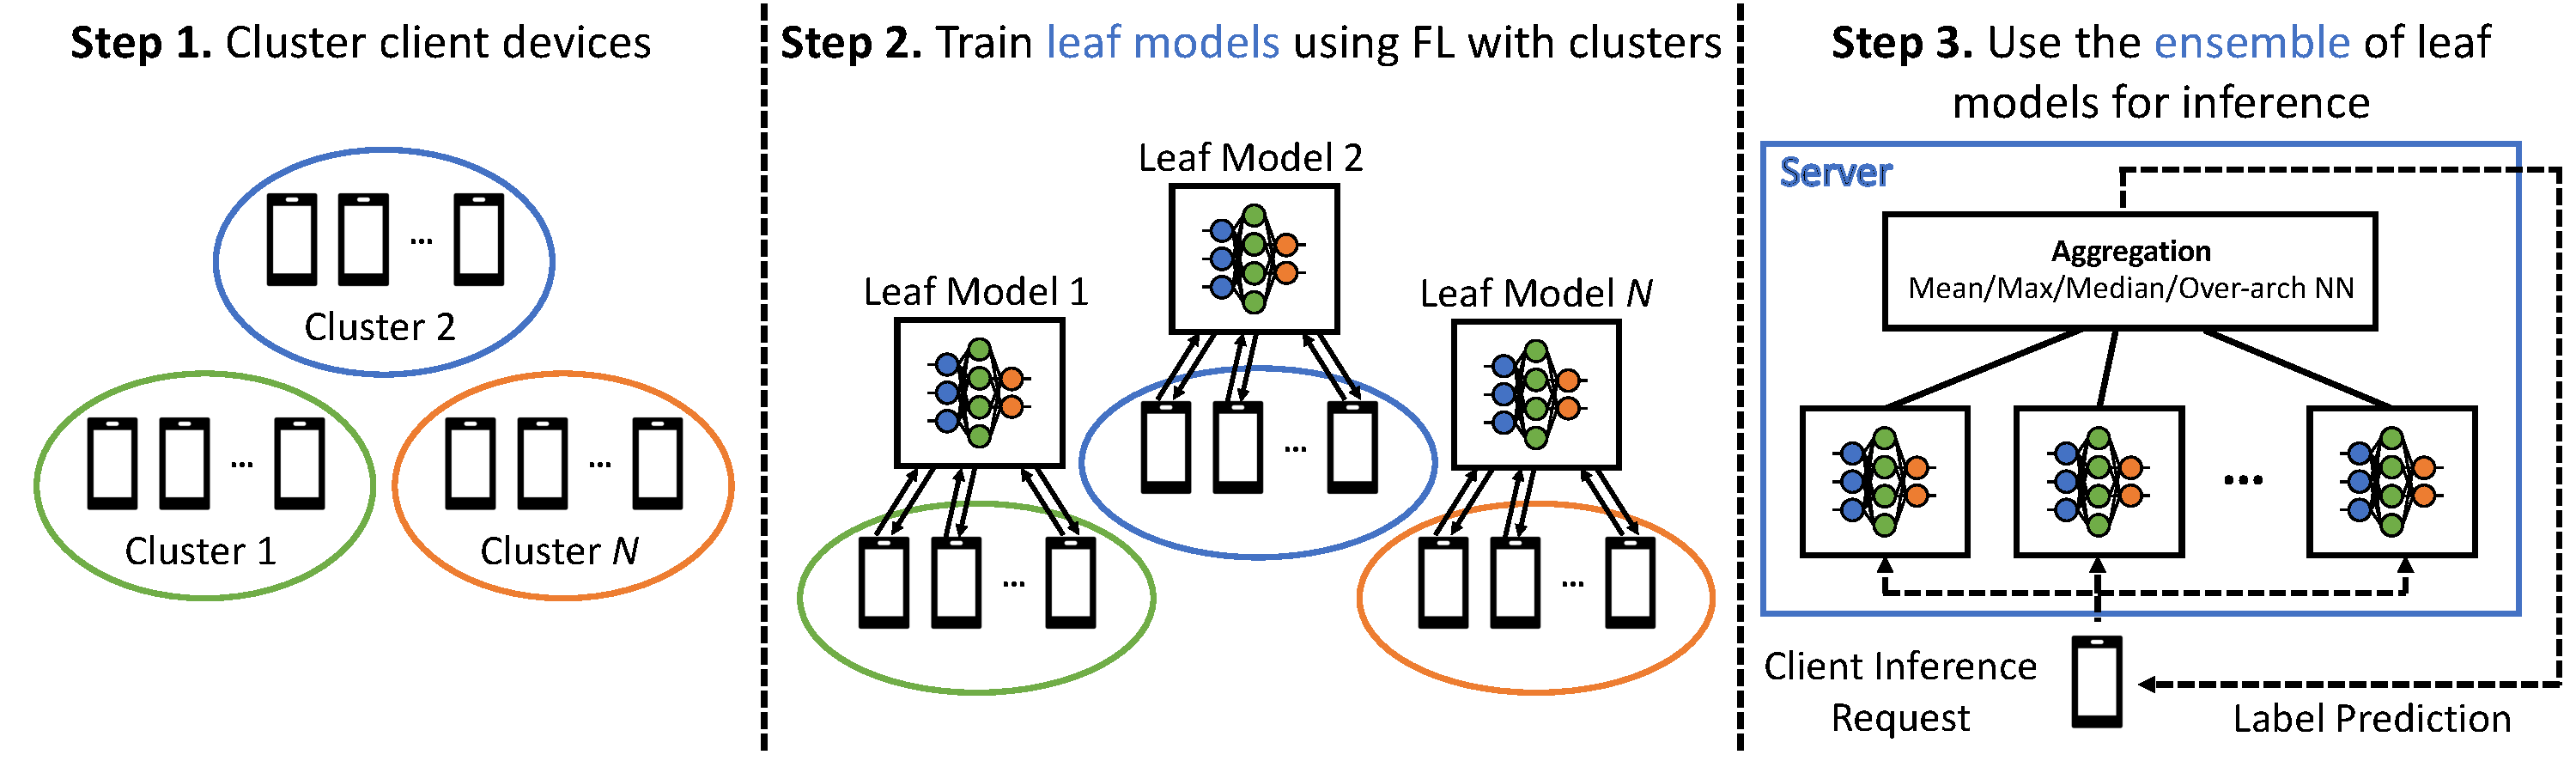
\includegraphics[width=1\textwidth]{submissions/ManiMalek/FEL2.pdf}
\vspace{-0.35cm}
\caption{\label{fig:FEL_architecture.png} Federated Ensemble Learning architectures}
\vspace{-0.35cm}
\end{figure}

\subsection{Privacy Analysis for Federated Ensemble Learning}
\vspace{-0.25cm}
\label{sec:privacy}
%\il{TODO: remind here that this is a key requirement and we are the first to do this analysis for FEL. Also maybe put this as section 4 (own section?}
Ensuring data privacy is the utmost requirement and this work is the first to conduct privacy analysis for federated ensemble learning.
Differential privacy for federated learning bounds how much the distribution of model parameters change between two datasets that differ in \emph{labels} contributed by a single user \cite{mcmahan2017learning}. We use a generalization of differential privacy~\cite{dwork2006calibrating} based on the R{\'e}nyi divergence:

\textbf{Definition 1} (Renyi Differential Privacy (RDP)~\cite{mironov2017renyi}). A \textit{randomized mechanism $\mathrm{M}$ with domain $\mathrm{D}$ is $(\alpha, \epsilon)$-RDP with order $\alpha \in (1,\infty)$ iff for any two neighboring datasets $D, D'\in \mathrm{D}$:}

\begin{align*}
  \mathrm{D}_\alpha(\mathrm{M}(D)||\mathrm{M}(D')):=\frac{1}{\alpha - 1}\log E_{x \sim \mathrm{M}(D')}\left[\left(\frac{\Pr[\mathrm{M}(D)=x]}{\Pr[\mathrm{M}(D')=x]}\right)^\alpha\right]\leq \epsilon.
\end{align*}

FEL is a multi-step process. To analyze the privacy bounds of a multi-step process, a common approach in differential privacy is to evaluate each process individually, then calculate the overall privacy bounds by composing all of the steps. In particular, we focus on two main composition theorems in differential privacy, sequential and parallel composition \cite{dwork2009differential}. Formally we define:


\textbf{Theorem 1} (Sequential Composition). \textit{Let there be n RDP-mechanisms $\mathrm{M}_i$ with $(\alpha, \epsilon_i)$-RDP when being computed on a dataset $D$ of the input domain $\mathrm{D}$. Then, the composition of n mechanisms $\mathrm{M}(\mathrm{M}_1(D),\dots,\mathrm{M}_n(D))$ is $(\alpha, \sum^n_{i=1} \epsilon_i)$-RDP}


\textbf{Theorem 2} (Parallel Composition). \textit{Let there be n RDP-mechanisms $\mathrm{M}_i$ with $(\alpha, \epsilon_i)$-RDP when being computed on disjoint subset $\mathrm{D}_i$ of the input domain $\mathrm{D}$. Then, the composition of n mechanisms $\mathrm{M}(\mathrm{M}_1(D),\dots,\mathrm{M}_n(D))$ is $(\alpha, \max^n_{i=1} \epsilon_i)$-RDP}

Sequential composition considers the case where a task uses the same users (even if different steps use different parts of the user’s data) in different steps of an algorithm. For example, if the algorithm has four steps each with a privacy cost $\eps$ and uses the same users in all the steps, the total privacy cost of the algorithm would become $4\eps$.
%
Parallel composition considers a case where each step is applied to different users. From the earlier example, if four disjoint sets of users were used for the four steps, the overall privacy cost would be $\max(\eps_1,\eps_2,\eps_3,\eps_4)$, where $\eps_k$ is the privacy cost of the $k$-th step. The compositions are tracked using RDP, which leads to tighter bounds than $(\epsilon, \delta)$-DP.
%We show some examples in this post and also please refer to [R2] for more details. Please note, while it is possible to do composition directly with DP, the bounds are not as tight as in RDP. Therefore, we chose RDP for the analysis.

When analyzing the privacy cost of training the leaf models, the parallel composition theorem applies as each leaf model is trained with a disjoint set of users. If training a leaf model with cluster $i \in \{1,\dots,N\}$ has a privacy cost $e_i$, the privacy cost of the entire leaf model is $e_\mathrm{leafs} = \max(e_1,\dots, e_N)$.

The privacy cost of the ensemble aggregation layer $e_\mathrm{agg}$ depends on the aggregation method that is used (mean, max, median, or NN-based).
When using the mean, max, and median ensemble aggregation, $e_\mathrm{agg}=0$ as both theorems show that privacy cost increases only when the additional step (ensemble aggregation) uses user data.
%
In this case, the total privacy cost $e_\mathrm{tot}$ is simply $e_\mathrm{leafs}$.


%
When the NN-based approach is used, however, user data is used to train the over-arch NN layer and $e_\mathrm{agg} > 0$. Depending on exactly how the over-arch NN layer is trained, $e_\mathrm{tot}$ can be calculated in the following way.
%
First, if the over-arch NN layer is trained with the users that trained the leaf models, sequential composition theorem applies ($e_\mathrm{tot} = e_\mathrm{agg} + e_\mathrm{leafs}$).
Second, if the over-arch NN layer is trained with a completely different set of users, the parallel composition theorem applies ($e_\mathrm{tot} = \max(e_\mathrm{agg}, e_\mathrm{leafs})$).
Finally, if the over-arch NN layer is trained with opt-in users, $e_\mathrm{agg}=0$ because no private data is used, and $e_\mathrm{tot}=e_\mathrm{leafs}$.
In all cases, the privacy cost of FEL does not significantly deteriorate over the vanilla FL (which is similar to $e_\mathrm{leafs}$).
%\end{itemize}

%is the only approach which uses user data to train an aggregation model. Similarly, we have two options to train the overarch model:

%\begin{itemize}
%\item If the overarch method uses a similar set of users as used in training the sub-models, then, we have to use the sequential composition, since by changing one user it will change the output of both sub-models and the aggregation model. If training the sub-models has privacy cost of $e_1$ and training the overarch model has privacy cost of $e_2$. The overall privacy costs will be $e_1+e_2$.
%\item If the overarch method uses a completely different set of users as used in training the sub-models, then, we use the parallel composition, since by changing one user it will only change the output of both sub-models or the aggregation model (not both). If training the sub-models has privacy cost of $e_1$ and training the overarch model has privacy cost of $e_2$. The overall privacy costs will be $\max(e_1,e_2)$.
%\item If the overarch method uses publicly available opt-in users data, the training of overarch does not have an additional privacy and the overall privacy cost is $e_1$.
%\end{itemize}

%Figure \ref{fig:FELPrivacy.png} summarizes this logic.

%\begin{figure}
%\centering
%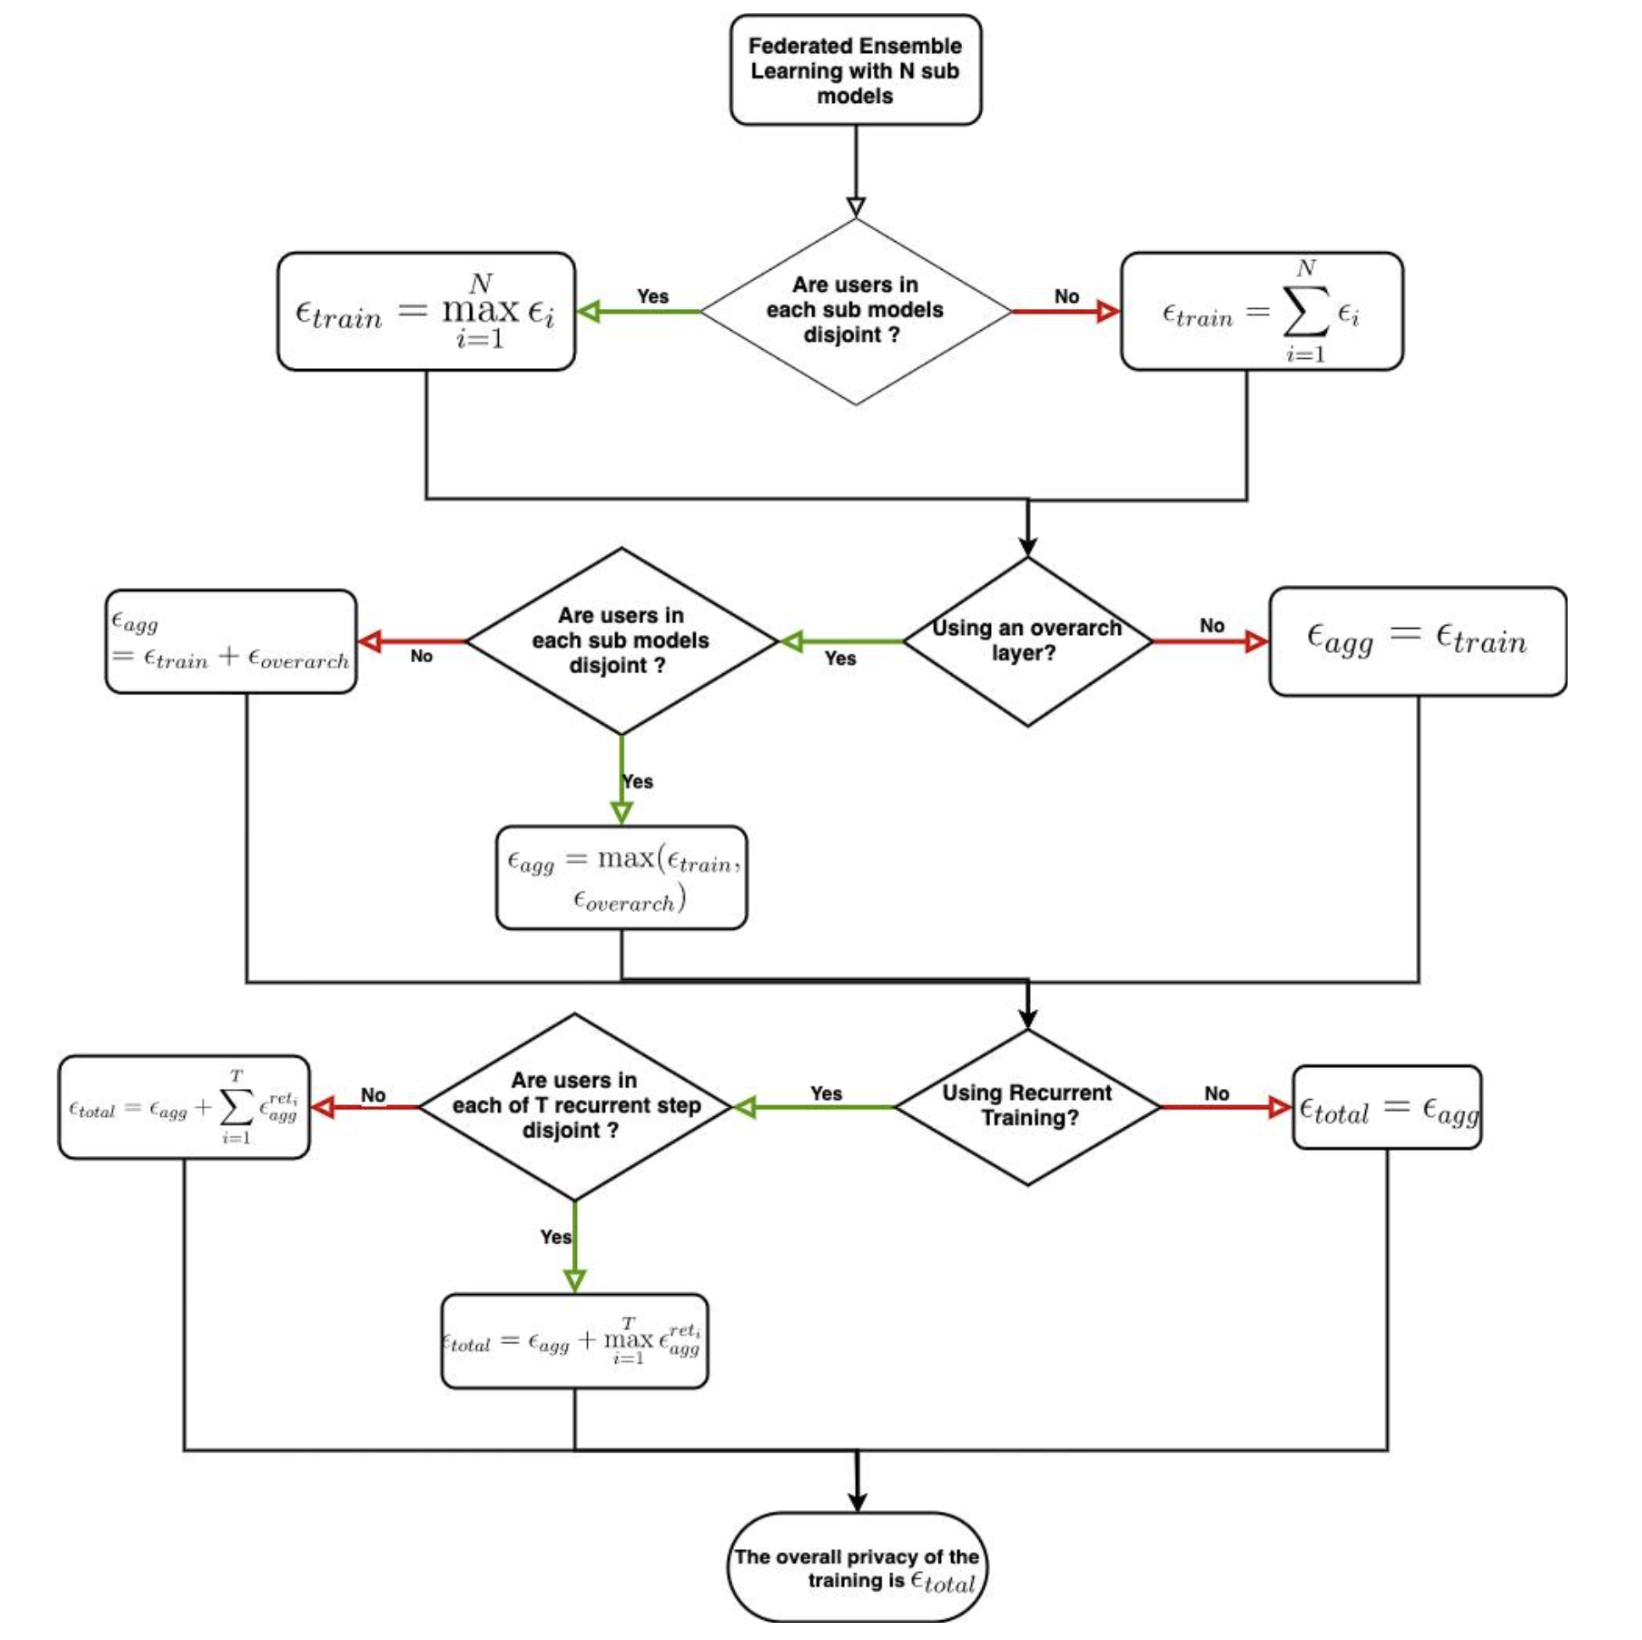
\includegraphics[width=1\textwidth]{FELPrivacy.png}
%\caption{\label{fig:FELPrivacy.png} Privacy analysis of Federated Ensemble Learning}
%\end{figure}




\section{Evaluation}
In this section we would like to provide more details about our experiments. We first provide details about each dataset that was used. We then provide details about the model architectures that we used for each dataset.
\subsection{Datasets for FEL}
\label{sec:datasets}
We explored three datasets for FEL: An internal production dataset that represents a real-world ads-ranking system, an external dataset that addresses a similar ads-ranking task, and an image classification dataset.

\subsubsection{Production Dataset}
Production dataset is an internal dataset that captures whether a user installs a mobile application after being shown a relevant advertisement item. A few hundred features are used as an input (the exact number cannot be disclosed) to predict a binary label (install/not-install). All the input features are public. For training, we use advertisement data from a random sample of 35 million users over a period of one month. Randomly selected 15 million users from the following week were used for testing.

%\subsection{Open-Source Datasets}

\subsubsection{Taobao CTR Dataset}
The Taobao dataset contains 26 million interactions (click/non-click when an Ad was shown) between 1.14 million users and 847 thousand items across an 8-day period.
The dataset uses 9 user features (e.g., gender or occupation), 6 item features (e.g., price or brand), and two contextual features (e.g., the day of week), which we assume to be all public to the service provider.

In the Taobao CTR dataset, 16 out of the 17 features are sparse, with a categorical value encoding instead of a continuous, floating point value.
%
While server-based recommendation models use large embedding tables to convert these sparse features into a floating point embedding~\cite{din, dlrm, wideanddeep}, training such embedding tables on device is complicated because of the large memory capacity requirement (e.g., in the order of GB to TB~\cite{zhao2020distributed,acun:2021:understandingtraining,wilkening:2021:recssd,lui:2021:capacity}) and can leak private information more easily through gradients~\cite{alibaba_fl}. %significantly~\cite{zhang2021wide}.
Thus, we assume an architecture where embedding tables are pre-trained with opt-in users and are hosted on the server, while the rest of the model is trained with FEL using sparse features translated through the pre-trained tables. We randomly selected 10\% of the users as opt-in.

Our setup cannot achieve the accuracy that can be reached when we fully train the embedding tables, as we pre-train the embeddings and fix their weight during FL.
However, our setup represents a practical FL setup where training embedding tables on-device is prohibitive, due to client resource limitations~\cite{nguyen2021federated} and privacy concerns~\cite{alibaba_fl}.




\subsubsection{CelebA Smile Prediction Dataset}
While FEL is originally designed for recommendation and ranking tasks, we study its generality to non-recommendation models with CelebFaces Attributes Dataset (CelebA)~\cite{liu2015deep}. CelebA consists of $200,288$ images belonging to $9,343$ unique celebrities. Each image has 40 binary facial attribute annotations (e.g., bald, long hair, attractive, etc) and covers large pose variations and backgrounds.
We defined distinguishing between smiling/non-smiling images as our target task.

The Taobao dataset contains 26 million interactions (click/non-click when an Ad was shown) between 1.14 million users and 847 thousand items across an 8-day period.
The dataset uses 9 user features (e.g., gender or occupation), 6 item features (e.g., price or brand), and two contextual features (e.g., the day of week), which we assume to be all public to the service provider. The details on how we preprocess the  dataset can be found in the appendix.




\subsection{Model Architectures}
{\bf Production/Taobao Dataset:}
For recommendation datasets (production/Taobao CTR), we use a model that consists of 3 fully-connected hidden layers. The number of units at each hidden layer is decreasing exponentially with a parameter K. For instance, if $K=4$ and the input layer has 512 features, our neural network would have  $[512, 128, 32, 8, 1]$ neurons. For each dataset, we tune K to obtain a resulting model of approximately $10$MB. By doing so, it allows us to train a neural network even on older, low-tier devices with more limited memory capacity. ReLu is used as an activation function after each layer apart from the last one, where Sigmoid and binary cross-entropy was used.

For both datasets, we use synchronous FL with FedAvg~\cite{mcmahan2017learning}. We used the following hyperparameters for the Taobao dataset from an extensive hyperparameter search: client batch size of 32, 5 local epochs, 4096 clients per round, and a learning rate of 0.579 with SGD. Clients are selected at random and each only participates once (1 global epoch). The production dataset used similar hyperparameters.

For Taobao dataset's server-side pre-trained embedding table, we use an embedding dimension of 32, and train it with the 10\% opt-in users for 1 epoch using AdaGrad optimizer with learning rate of 0.01.

{\bf CelebA Dataset:}
For CelebA, we follow the setup of prior work~\cite{nguyen2021federated} and use a four layer CNN with dropout rate of 0.1, stride of 1, and padding of 2. We preprocess all images in train/validation/test sets; each image is resized and cropped to 32$\times$32 pixels, then normalized by 0.5 mean and 0.5 standard deviation. We use asynchronous FL with a client batch size of 32 samples, 1 local epoch, 30 global epochs, and a learning rate of 0.899 with SGD.

\subsection{Evaluation Methodology}
\label{sec:appendix-b}
Our evaluation aims to answer the following questions:

\begin{itemize}
    \item Can FEL improve the model prediction quality over vanilla FL? [Section~\ref{sec:prediction-quality}]
    \item How do different ensemble aggregation methods affect the model accuracy? [Section~\ref{sec:prediction-quality}]
    \item How do different clustering methods affect the model accuracy? [Section~\ref{sec:prediction-quality-clustering}]
    \item How does FEL affect privacy compared to vanilla FL? [Section~\ref{sec:privacy-eval}]
\end{itemize}

To answer these questions we used the three datasets presented in Section~\ref{sec:datasets}. To study recommendation and ranking tasks, we used a production dataset and an open-source, Taobao's Click-Through-Rate (CTR) prediction dataset~\cite{li2021novel}.
To study the effect of FEL on non-recommendation use-cases, we additionally studied the LEAF CelebA Smile Prediction dataset~\cite{liu2015deep}. More details about these datasets and their associated model architecture can be found in Section~\ref{sec:datasets}.


Both the FL baseline and the FEL leaf models used the same set of hyperparameters.
The FL baseline is trained using all the available client data. In FEL, the client data is clustered, and one leaf model is trained for each cluster. We vary the number of clusters from 3--10 and evaluate different clustering methods.
When training the over-arch NN layer, a small subset of opt-in users is used.


\begin{table}
\small
\centering
\caption{\label{tab:clusterconfig} Explanation of different cluster methods in Figure~\ref{fig:eval0} (right).}
\begin{tabular}{|l||l|l|c|}
\hline
Dataset & Config & Feature & \# clusters \\ \hline\hline
\multirow{4}{*}{Production} & Clustering 1 & Age & 5\\
 & Clustering 2 & App & 5\\
 & Clustering 3 & Location & 4\\
 & Clustering 4 & Click ratio & 10\\\hline
\multirow{3}{*}{Taobao~\cite{taobao}} & Clustering 1 & Age & 7\\
 & Clustering 2 & Consumption & 4\\
 & Clustering 3 & City level & 5\\\hline
\multirow{3}{*}{CelebA~\cite{liu2015deep}} & Clustering 1 & \# Attributes & 3\\
 & Clustering 2 & K-means & 3\\
 & Clustering 3 & K-means & 5\\\hline
\end{tabular}\\
\end{table}



\subsection{Prediction Quality Improvement of FEL}
\vspace{-0.25cm}
\label{sec:prediction-quality}
Overall, FEL achieves \textbf{0.43\%} and \textbf{2.31\%} prediction quality improvement over vanilla FL for production and Taobao datasets, respectively -- a significant improvement for ranking and recommendation system use cases\footnote{\cite{zhao2020distributed} mentioned 0.1\% model quality improvement as significant and \cite{wang2017deep} considered 0.23\% as impactful in similar recommendation and ranking use-cases.}.
For non-recommendation tasks (CelebA), FEL shows similar improvement of~\textbf{1.55\%}, indicating that FEL can be generalized to non-recommendation use-cases as well.
Table~\ref{tab:result1} summarizes the resulting prediction quality improvement of FEL compared to the baseline FL. We used accuracy for CelebA~\cite{nguyen2021federated} and ROC-AUC (AUC) for Taobao~\cite{taobao}. We used normalized entropy for the production dataset, which we cannot disclose and only show the relative improvement.
For different ensemble aggregation methods, we vary the clustering methods and report the best-accuracy results.
Among the different ensemble aggregation methods, adding an over-arch NN layer provided the best prediction quality improvement, followed by mean and median.
%Max only showed improvement in CelebA and did not show benefit in recommendation use-cases.
%



\begin{table}
\centering
\caption{\label{tab:result1} FEL's prediction accuracy improvement over the baseline FL for different datasets. Following common practice of each dataset, Taobao uses AUC and CelebA uses accuracy as their metric. Production data's baseline accuracy is not disclosed.}
\begin{tabular}{|l|ccc|}
\hline
 & Production & Taobao~\cite{taobao} AUC & CelebA~\cite{liu2015deep} accuracy
 \\ \hline\hline

Baseline FL & - & 0.5418~\tablefootnote{Taobao's baseline AUC is 0.26\% less than the baseline FL result presented at~\cite{alibaba_fl}, potentially due to simpler model architecture and freezed pre-trained embedding tables.} & 90.75 \\\hline
FEL (Mean Best) & (+0.27\%) & 0.5522 (+1.92\%) & 91.68 (+1.02\%) \\
FEL (Median Best) & (+0.29\%) & 0.5459 (+0.74\%) & 91.35 (+0.66\%) \\
FEL (Max Best) & (-0.06\%) & 0.5418 (-0.1\%) & 91.46 (+0.78\%)\\
FEL (NN-based Best) & \textbf{(+0.43\%)} & \textbf{0.5544 (+2.31\%)} & \textbf{92.16 (+1.55\%)} \\\hline
\end{tabular}\\
\end{table}



\subsection{Prediction Quality Improvement of Different Clustering Methods}
\vspace{-0.25cm}
\label{sec:prediction-quality-clustering}

\begin{figure}
\centering
    \begin{subfigure}[]{
        \centering
        \includegraphics[width=0.45\textwidth]{submissions/ManiMalek/random_vs_partitions (1).pdf}
        %\caption{}
        \label{fig:eval0_0}
        }
     \end{subfigure}
     \begin{subfigure}[]{
        \centering
        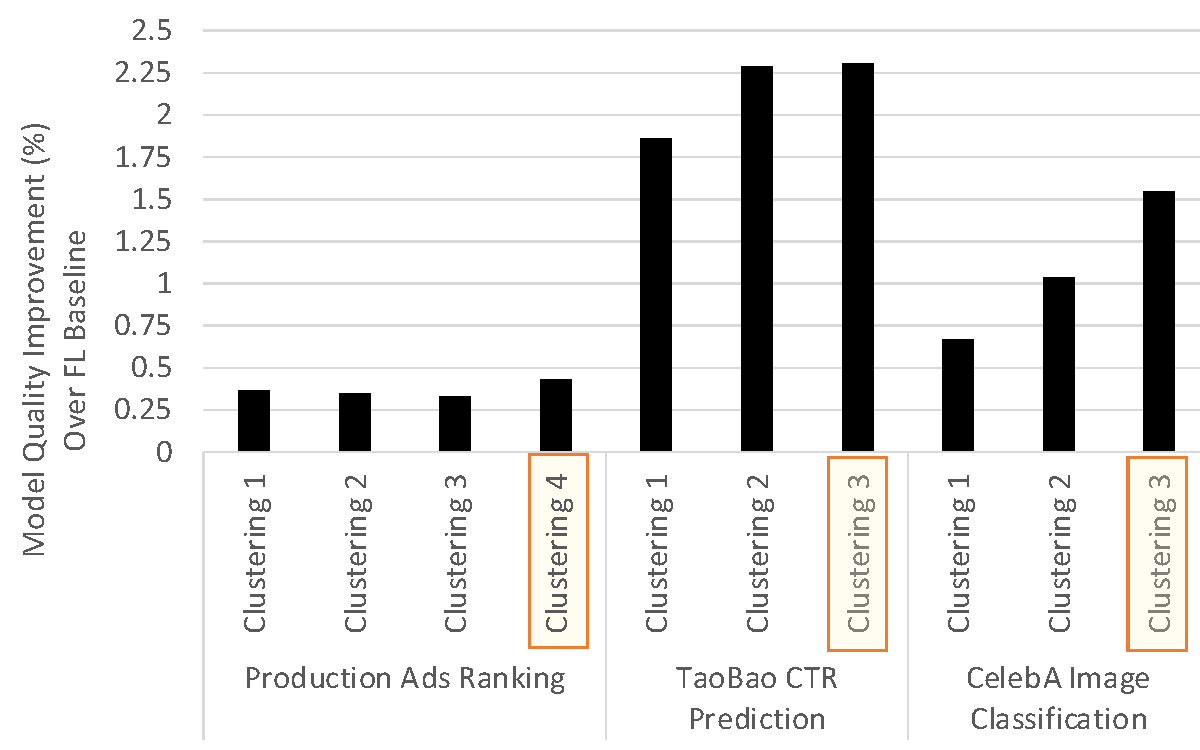
\includegraphics[width=0.49\textwidth]{submissions/ManiMalek/FEL.pdf}
        %\caption{}
        \label{fig:eval0_1}
        }
     \end{subfigure}
     \vspace{-0.3cm}
     \caption{Accuracy improvement for different number of clusters (segments) for each ensemble aggregation method (left), and different clustering methods when using over-arch NN layer (right). Different clustering methods are explain in Table~\ref{tab:clusterconfig}}
    \label{fig:eval0}
%\includegraphics[width=0.4\textwidth]{random_vs_partitions (1).pdf}
%\caption{\label{fig:eval0} Number of random segments vs. lift over the large FL baseline (Taobao dataset)}
\vspace{-0.25cm}
\end{figure}




{\bf Effects of the Number of Clusters:}
To understand the effect of the number of client clusters in the final model quality improvement, we varied the number of clusters in the Taobao dataset while using random clustering.
%
Figure~\ref{fig:eval0} (left) summarizes the result. There is an optimal setting for the number of clusters used in FEL. Going beyond the optimal setting for the number of clusters results in worse model accuracy. When the number of clusters is too small, the final model capacity is limited as there are not enough leaf models to ensemble. If the number of clusters is too large, each leaf model cannot learn enough information as the clients in each cluster are too few. The optimal number of clusters depends on the number of available devices that participate within each cluster and, here, the number of partitions can be treated as a hyperparameter~\cite{kim:micro21}.

{\bf Effects of Features Used in Clustering:}
We also varied the clustering methods for each dataset and observed the effect on the final accuracy. We explored different clustering methods for different datasets and presented the best performing methods. Table~\ref{tab:clusterconfig} (Section~\ref{sec:appendix-b}) summarizes the clustering methods. Here, we show the result for the best performing over-arch NN-based ensemble aggregation for brevity. For the production dataset, we used user age, the app category where the ad was displayed, location (larger geographic regions), and previous click ratio of the users to cluster the users. For Taobao, we used user age, city level, and consumption level. For CelebA, we clustered the 40 binary attributes of each user using K-means clustering or simply used the number of present attributes.


Figure~\ref{fig:eval0} (right) shows that clustering can affect the final model accuracy significantly. For the production dataset, clustering using the click ratio (Clustering 4) showed the best accuracy. For Taobao, clustering with city level showed the best accuracy (Clustering 3). For CelebA, using K-means clustering was the best (Clustering 3). The results show that clustering methods as well as the number of clusters are two important hyperparameters of FEL.

%\begin{figure*}
%\centering
%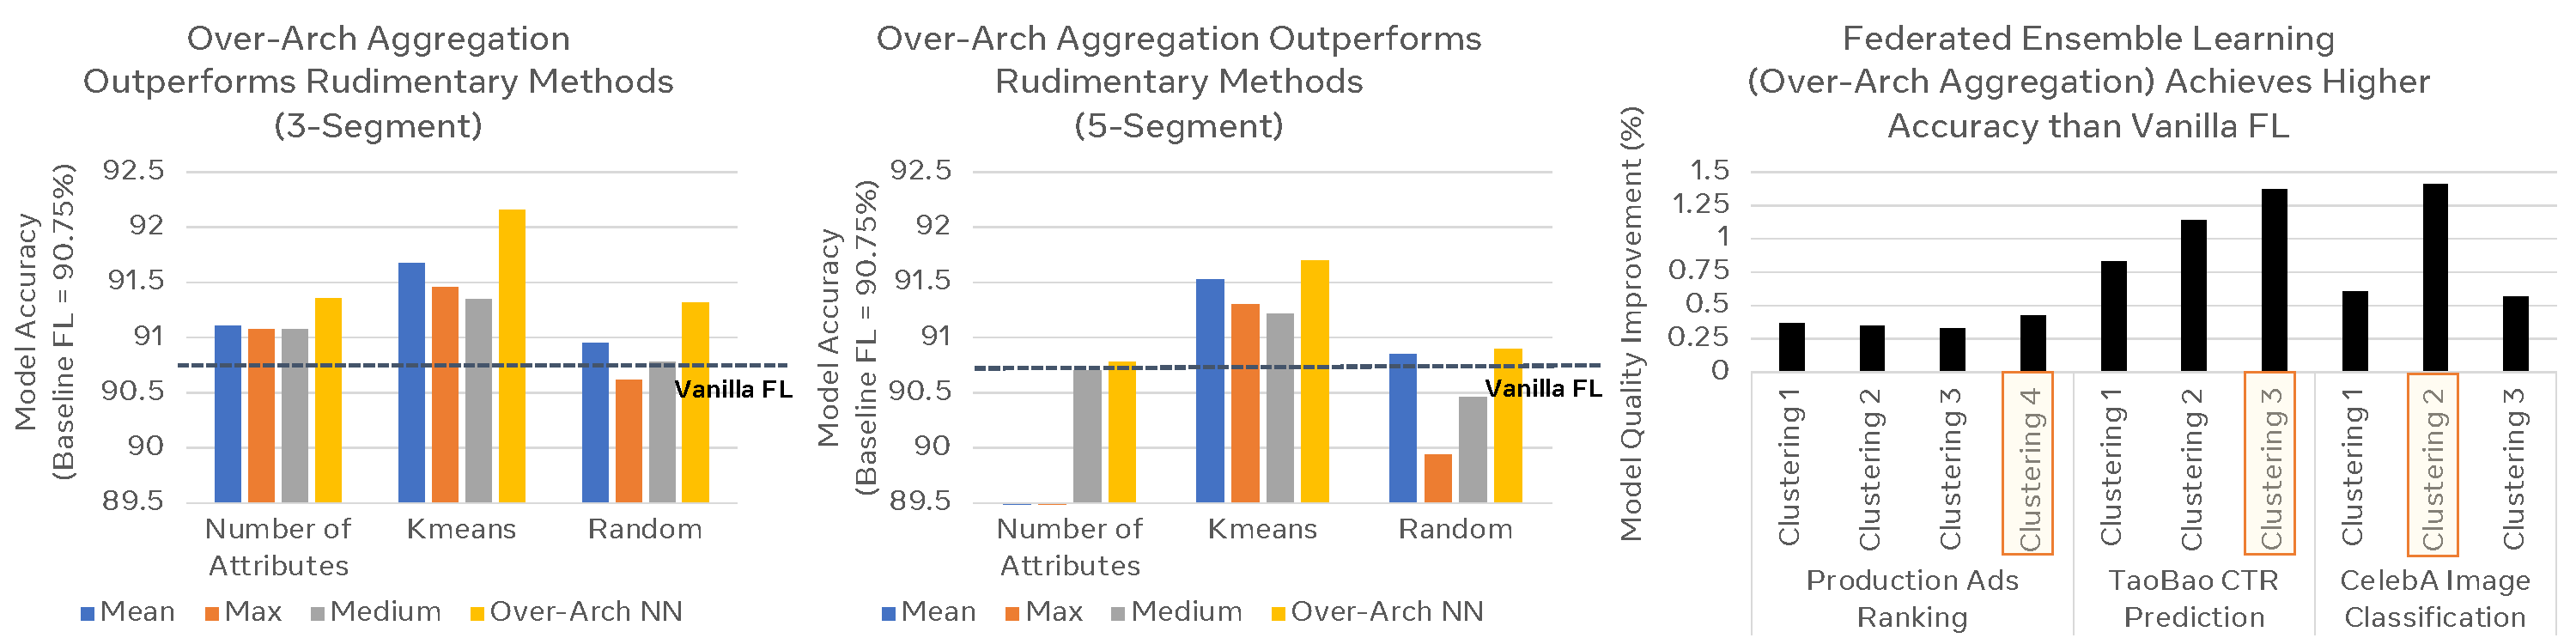
\includegraphics[width=1\textwidth]{FEL-result.pdf}
%\caption{\textcolor{blue}{Result Overview}}
%\end{figure*}


%\subsection{Number of Sub-Models}

%To evaluate the benefits of increased model capacity through the number of parameters, we split the training data into random partitions and train a leaf model within each partition. While each device only trains a small, 10 megabyte (MB) leaf model, the ensemble can reach hundreds of MBs. Here, each part of the ensemble will be trained on a subset of the entire dataset.

%Figure~\ref{fig:part_number} illustrates the model accuracy improvement results over the number of segments for the Taobao CTR dataset. Increasing model capacity through FEL achieves accuracy improvement as long as the training sub-partitions contain enough data to train the leaf models. In this dataset, we only had 900 thousand users participating at FL. Splitting the population into more than 15 partitions results in too few users per leaf to fully train a model. The optimal number of partitions depends on the number of available devices that participate within each cluster and, therefore, the number of partitions can be treated as a hyperparameter~\cite{kim:micro21}.

%With respect to the ensemble aggregation strategies, the \emph{mean} aggregation results in significant quality improvement over the federated learning baseline, by up to 1.32\%. The  overarching neural network architecture results in slightly improved performance with an accuracy increase of 1.38\% but it requires opt-in data for model training.

%\subsection{Segment-Specific Leaf Models}
%In addition to random partitions that can result in increased learning capacity for FL over resource-constrained devices, we also explore creating leaf models for specific user or device segments.

%\subsubsection{Evaluation Results for CelebA}
%In addition to ranking and recommendation tasks, we evaluate FEL using an image classification dataset with a balanced label distribution. We use prediction accuracy as the performance metric.
%We train our models using the same convolutional network classifier in~\cite{nguyen2021federated} and use non Independent and Identically Distributed (IID) client partitions for the federated learning training as described in~\cite{nguyen2021federated}. We use a batch size of 32.

%We rely on the 40 binary metadata attributes to partition the user population into disjoint segments. In the first method, we construct a numerical feature by counting the number of attributes for each image, and then use this feature to partition the data into segments.
%In addition, in the second method, we build partitions by applying K-means clustering to the matrix of binary attributes. We vary the number of segments from 3 to 5 and also show the results for random segments as well.

%Table~\ref{tab:FELcelebAResults} shows that FEL can consistently outperform the large-capacity FL baseline. FEL achieves higher accuracy gains with the 3-segment settings while the gains are moderate for the 5-segment settings. Both custom segmentation methods outperform random segments.

\begin{comment}
\begin{table}
\centering
\begin{tabular}{lccc}
\hline
Model & Aggregation & Accuracy & \%  lift on baseline \\ \hline\hline
FL Large baseline &  & 90.75 & 0.00 \\ \hline
%  &  &  &  \\
& Mean  & 91.11 & 0.39 \\
Num. Attributes (3 segments)                  & Max  & 91.08 & 0.36 \\
 & Median  & 91.08 & 0.36 \\
 & NN & 91.36 & \textbf{0.67} \\ \hline
%  &  &  &  \\
& Mean  & 89.22 & -1.69 \\
Num. Attributes (5 segments)  & Max  & 85.01 & -6.33 \\
 & Median  & 90.7 & -0.06 \\
 & NN & 90.78 & \textbf{0.03} \\ \hline
%  &  &  &  \\
& Mean  & 91.68 & 1.02 \\
Kmeans (3 segments)  & Max  & 91.46 & 0.78 \\
 & Median  & 91.35 & 0.66 \\
 & NN & 92.16 & \textbf{1.55} \\ \hline
%  &  &  &  \\
& Mean  & 91.53 & 0.86 \\
Kmeans (5 segments)  & Max  & 91.3 & 0.60 \\
 & Median  & 91.22 & 0.52 \\
 & NN & 91.70 & \textbf{1.04} \\ \hline
%  &  &  &  \\
& Mean  & 90.95 & 0.22 \\
Random (3 segments)  & Max  & 90.62 & -0.14 \\
 & Median  & 90.78 & 0.03 \\
 & NN & 91.32 & \textbf{0.63} \\ \hline
%  &  &  &  \\
& Mean  & 90.85 & 0.10 \\
Random (5 segments)  & Max  & 89.94 & -0.90 \\
 & Median  & 90.46 & -0.33 \\
 & NN & 90.90 & \textbf{0.16} \\ \hline
\end{tabular}
\caption{\label{tab:FELcelebAResults} Results of FEL experiment on CelebA dataset}
\end{table}


\subsubsection{Evaluation Results for Production Recommendation and Ranking}


\begin{table}
\centering
\begin{tabular}{|l|cccc|}
\hline
Model  &  Max & Median & Mean & NN  \\ \hline\hline

Production - Age (5 segments)      & -0.7  & 0.29 & 0.25 & \textbf{0.37}\\\hline
Production - App (5 segments).     & -3.4  & 0.10 & 0.03 & \textbf{0.35}\\\hline
Production - Location (3 segments) & -0.06 & 0.21 & 0.27 & \textbf{0.33}\\\hline
Production - Click ratio (10 segments) & -0.91 & 0.28 & 0.27 & \textbf{0.43} \\ \hline
Taobao - Age (7 segments)         & -0.10 & -0.23 & 1.27 & \textbf{1.86} \\ \hline
Taobao - Consumption (4 segments) &-1.64 & -0.46 & 1.92 & \textbf{2.29} \\ \hline
Taobao - City level (5 segments)  & -2.07 & 0.74 & 1.86 & \textbf{2.31} \\ \hline
\end{tabular}\\
\caption{\label{tab:FEAdsResults} Results of FEL on ad prediction datasets (percentage gain over the large FL baseline). Gains over 0.2\% are considered significant in this scenario. \textcolor{red}{Ilias: This number (gains over 0.2 are significant) needs to be justified/discussed. I just put it as a placeholder. Alternatively we can remove it (if we cannot justify it)}.}
\end{table}


Table~\ref{tab:FEAdsResults} shows the results of FEL on the two ad-ranking datasets. Note only the FEL lift over the FL baseline is presented as we cannot disclose the actual precision for the internal production baselines.
For both datasets, these results demonstrate the importance of selecting features that segment the user base into meaningful partitions. Training the  \emph{NN} overarching architecture provides the highest lift whereas the \emph{mean} aggregation strategy is a good alternative if no opt-in data are available. In our internal production dataset FEL provided a lift of up to 0.43\% that is considered \emph{significant in our domain}. In the taobao dataset the lift was even higher as the original FL baseline and the input features are not as optimised.
\end{comment}

\subsection{Evaluation Results with Differential Privacy}
\vspace{-0.25cm}
\label{sec:privacy-eval}

\begin{table}
\centering
\caption{\label{tab:FEAdsResultsDP} Taobao dataset with DP. Percentage of FEL's accuracy improvement over the FL baseline with the same level of DP noise is shown. Table~\ref{tab:clusterconfig} explains the clustering configurations.}
%\begin{tabular}{|lcc|cccc|}
\begin{tabular}{|lc|cccc|}
\hline
Config & $\epsilon$ & Mean & Median & Max & Over-Arch NN  \\ \hline\hline
\multirow{3}{*}{Clustering 1} & $\infty$ & +1.27\% & -0.23\% & -0.10\% & \textbf{+1.86\%} \\
 & 3.78 & +0.63\% & -0.14\% & +0.11\% & \textbf{+0.66\%} \\
 & 1.56 & +0.32\% & -0.23\% & +0.34\% & \textbf{+0.68\%} \\ \hline

\multirow{3}{*}{Clustering 2} & $\infty$ & +1.92\% & -0.46\% & -1.64\% & \textbf{+2.29\%} \\
 & 3.78 & +0.75\% & -0.21\% & +0.03\% & \textbf{+1.38\%} \\
 & 1.56 & +0.69\% & -0.11\% & +0.74\% & \textbf{+0.76\%} \\ \hline

\multirow{3}{*}{Clustering 3} & $\infty$ & +1.86\% & +0.74\% & -2.07\% & \textbf{+2.31\%} \\
 & 3.78 & +1.49\% & -0.09\% & +1.03\% & \textbf{+1.93\%} \\
 & 1.56 & +0.71\% & -0.37\% & +1.26\% & \textbf{+1.02\%} \\ \hline

%Model & DP Noise & $\epsilon$ & Max & Median & Mean & NN  \\ \hline\hline
%Age         & 0.7 & 3.78 & 0.11 & -0.14 & 0.63 & \textbf{0.66} \\ \hline
%Consumption & 0.7 & 3.78 & 0.03 & -0.21 & 0.75 & \textbf{1.38} \\ \hline
%City level  & 0.7 & 3.78 & 1.03 & -0.09 & 1.49 & \textbf{1.93} \\ \hline\hline
%Age         & 1 & 1.56 & 0.34 & -0.23 & 0.32 & \textbf{0.68} \\ \hline
%Consumption & 1 & 1.56 & 0.74 & -0.11 & 0.69 & \textbf{0.76} \\ \hline
%City level  & 1 & 1.56 & 1.26 & -0.37 & 0.71 & \textbf{1.02} \\ \hline
\end{tabular}\\
\vspace{-0.25cm}
\end{table}

%\textcolor{red}{Luca: I would drop the DP noise from the table, epsilon is enough }
%\textcolor{red}{Ilias: Placeholder text, we could expand/improve:}
Table~\ref{tab:FEAdsResultsDP} shows the accuracy improvement of FEL compared to vanilla FL for two different levels of DP noise, along with the case of no DP noise ($\epsilon=\infty$). We assume the over-arch NN layer was trained with opt-in data and no DP noise added when training the over-arch NN layer.
Table~\ref{tab:FEAdsResultsDP} shows that even when DP noise is added, FEL shows meaningful accuracy improvement over vanilla FL.
Again, we observe that the over-arch NN layer and mean aggregations still provide the most significant gains.
However, smaller $\epsilon$ leads to reduced accuracy gain, possibly due to larger injected noise.
%\textcolor{red}{Kiwan: Do we have an explanation for this? Luca: smaller eps -> higher privacy regime -> larger noise applied}.
%
Another interesting observation is that the max ensemble aggregation improves the accuracy when DP noise is added, unlike the no-DP-noise case where it did not show any improvement. One possible reason is that DP noise mitigates the effects of outliers in training.
%\textcolor{red}{Ilias: should we hypothesise why here? Luca: Maybe because DP mitigates the effects of the outliers in the dataset?}.


\section{Related Work}
\vspace{-0.25cm}
%This study resides in the intersection of four areas of study: ensemble distillation, boosted federated learning, local ensemble learning, and ensemble aggregation.

\textbf{Ensemble Distillation.} Lin et al.~\cite{lin2020ensemble} relied on unlabeled data generated by a generative model to aggregate knowledge from all heterogeneous client models, %, rather than leveraging FedAVG. and use average logit and fusion to share learning between heterogeneous models.
Gong et al.~\cite{gong2022preserving} focused on communication efficiency and privacy guarantee with one-shot offline knowledge distillation. %This proposal keeps the local training asynchronous and independent, and then aggregates the local predictions on unlabeled cross-domain public data.
%Sui et al.~\cite{sui2020feded} explore a knowledge distillation strategy which uses the uploaded predictions of ensemble local models to train the central model without requiring uploading local parameters. This approach only uses predicted labels on a small dataset to learn a student model from an ensemble of multiple local teacher models.

\textbf{Boosted Federated Learning.} Boosting and bagging are two prominent approaches for model ensemble learning.
%Li et al.~\cite{li2020practical} distribute data samples with the same features among multiple parties, relaxing privacy concerns.%. In their approach, each party boosts a number of trees by exploiting similarity information based on locality-sensitive hashing.
In Hamer et al.~\cite{hamer2020fedboost}, an ensemble of pre-trained based predictors is fine tuned via federated learning, thus saving on communication costs. Luo et al.~\cite{luo2021research} suggest gradient boosting decision tree (GBDT) method, which takes the average gradient of similar samples and its own gradient as a new gradient to improve the accuracy of the local model.

\textbf{Local Ensemble Learning.}
FedEnsemble uses random permutations to update a group of $K$ models, and then obtains predictions through model averaging, instead of aggregating local models to update a single global model~\cite{shi2021fed}. %Similarly, Majeed et al.~\cite{majeed2020blockchain} suggest an ensemble learning FL regime in which five base FL models are trained using the same local datasets, and ensemble using simple majority voting rule.
Attota et al.~\cite{attota2021ensemble} propose a multi-view ensemble learning approach aimed at maximizing the learning efficiency of different classes of attacks for intrusion detection tasks.

\textbf{Ensemble Aggregation.} FedBE takes a Bayesian inference perspective by sampling and combining higher-quality global models via Bayesian ensemble for robust aggregation~\cite{chen2020fedbe}.
%Guha et al.~\cite{guha2019one} propose one-shot learning, where a central server learns a global model over a network of federated devices in a single round of communication.
FedGRU uses both secure parameter aggregation and cluster ensembles to scale~\cite{liu2020privacy}.  %Bian et al.~\cite{bian2021fedseal} extend federated ensembles to the context of semi-supervised learning, leveraging self-ensembles, to enable clients to label their own data.
Orhobor et al.~\cite{orhobor2020federated} assigned users into pre-specified bins and trained different regressors on each bin, which were later ensembled.

Although these methods have their own merits, they do not address the problem of the recommender and ranking systems use cases, in which each user has only a small number of examples, and require user-level privacy guarantee. As a result, none of these studies leverages the variation across users and diversity of behavior in their proposals. Our approach trains models on separate user clusters,
% users and trains different models on different users,
leveraging a large user base in recommender and ranking systems.
Furthermore, our over-arch model approach provides extra gains both in terms of precision and privacy budget.


\section{Conclusion}
\vspace{-0.25cm}
While Federated learning (FL) has achieved considerable success as a privacy-preserving solution for model training, its impact on ranking and recommendation systems, particularly in the context of digital advertising, remains limited. We introduce Federated Ensemble Learning (FEL) to increases the learning capacity of FL.
% FEL clusters client population and trains a leaf model per each cluster, which are later ensembled to form a larger inference model.
FEL can be trained efficiently without introducing significant privacy concerns and can improve the prediction accuracy meaningfully compared to vanilla FL.
This work demonstrates that FEL enables FL for demanding ranking and recommendation tasks.
% As future work we plan  to evaluate FEL on different model architectures, such as transformer, LSTM, RNN, or CNN and on other tasks such as speech recognition, reinforcement learning,  etc.
%
As future work, we plan to integrate unsupervised clustering approaches, so that the segmentation can happen automatically to optimize FEL's learning performance.
%While this approach might provide better precision, it might create difficulty in productionizing FEL.
%
Finally, to minimize the cost of managing a number of leaf models, we plan to explore ways to automatically assess the quality of leaf models to pinpoint under-represented clusters and seek possible mitigation such as dynamic clustering and leaf retraining.
%An under-represented cluster can potentially The other extension could be to resort to a teacher-student setting where users with big groups can help improve the model of users in smaller groups.



%\bibliographystyle{abbrv}
%\bibliography{submissions/ManiMalek/sample}

\begin{thebibliography}{10}

\bibitem{abdulrahman2020survey}
S.~AbdulRahman, H.~Tout, H.~Ould-Slimane, A.~Mourad, C.~Talhi, and M.~Guizani.
\newblock A survey on federated learning: The journey from centralized to
  distributed on-site learning and beyond.
\newblock {\em IEEE Internet of Things Journal}, 8(7):5476--5497, 2020.

\bibitem{acun:2021:understandingtraining}
B.~Acun, M.~Murphy, X.~Wang, J.~Nie, C.-J. Wu, and K.~Hazelwood.
\newblock Understanding training efficiency of deep learning recommendation
  models at scale.
\newblock In {\em 2021 IEEE International Symposium on High Performance
  Computer Architecture (HPCA)}, 2021.

\bibitem{attota2021ensemble}
D.~C. Attota, V.~Mothukuri, R.~M. Parizi, and S.~Pouriyeh.
\newblock An ensemble multi-view federated learning intrusion detection for
  {IoT}.
\newblock {\em IEEE Access}, 9:117734--117745, 2021.

\bibitem{beane1987market}
T.~Beane and D.~Ennis.
\newblock Market segmentation: a review.
\newblock {\em European journal of marketing}, 1987.

\bibitem{secagg2017}
K.~Bonawitz, V.~Ivanov, B.~Kreuter, A.~Marcedone, H.~B. McMahan, S.~Patel,
  D.~Ramage, A.~Segal, and K.~Seth.
\newblock Practical secure aggregation for privacy-preserving machine learning.
\newblock In {\em Proceedings of the 2017 ACM SIGSAC Conference on Computer and
  Communications Security}, page 1175–1191, 2017.

\bibitem{expanding_reach}
S.~Caldas, J.~Kone{\v{c}}ny, H.~B. McMahan, and A.~Talwalkar.
\newblock Expanding the reach of federated learning by reducing client resource
  requirements.
\newblock {\em arXiv preprint arXiv:1812.07210}, 2018.

\bibitem{chen2020fedbe}
H.-Y. Chen and W.-L. Chao.
\newblock {FedBE}: Making {B}ayesian model ensemble applicable to federated
  learning.
\newblock {\em arXiv preprint arXiv:2009.01974}, 2020.

\bibitem{wideanddeep}
H.-T. Cheng, L.~Koc, J.~Harmsen, T.~Shaked, T.~Chandra, H.~Aradhye,
  G.~Anderson, G.~Corrado, W.~Chai, M.~Ispir, et~al.
\newblock Wide \& deep learning for recommender systems.
\newblock In {\em Proceedings of the 1st workshop on deep learning for
  recommender systems}, pages 7--10, 2016.

\bibitem{heterofl}
E.~Diao, J.~Ding, and V.~Tarokh.
\newblock {HeteroFL}: Computation and communication efficient federated
  learning for heterogeneous clients.
\newblock In {\em 9th International Conference on Learning Representations,
  {ICLR} 2021, Virtual Event, Austria, May 3-7, 2021}. OpenReview.net, 2021.

\bibitem{dwork2009differential}
C.~Dwork and J.~Lei.
\newblock Differential privacy and robust statistics.
\newblock In {\em Proceedings of the forty-first annual ACM symposium on Theory
  of computing}, pages 371--380, 2009.

\bibitem{dwork2006calibrating}
C.~Dwork, F.~McSherry, K.~Nissim, and A.~Smith.
\newblock Calibrating noise to sensitivity in private data analysis.
\newblock In {\em Theory of Cryptography: Third Theory of Cryptography
  Conference, TCC 2006, New York, NY, USA, March 4-7, 2006. Proceedings 3},
  pages 265--284. Springer, 2006.

\bibitem{geyer2017}
R.~C. Geyer, T.~Klein, and M.~Nabi.
\newblock Differentially private federated learning: {A} client level
  perspective.
\newblock {\em CoRR}, abs/1712.07557, 2017.

\bibitem{ghazi2021deep}
B.~Ghazi, N.~Golowich, R.~Kumar, P.~Manurangsi, and C.~Zhang.
\newblock Deep learning with label differential privacy.
\newblock In {\em Advances in Neural Information Processing Systems (NeurIPS)},
  2021.

\bibitem{gong2022preserving}
X.~Gong, A.~Sharma, S.~Karanam, Z.~Wu, T.~Chen, D.~Doermann, and A.~Innanje.
\newblock Preserving privacy in federated learning with ensemble cross-domain
  knowledge distillation.
\newblock 2022.

\bibitem{movielens}
Grouplens.
\newblock {MovieLens} {20M} dataset, 2016.

\bibitem{hamer2020fedboost}
J.~Hamer, M.~Mohri, and A.~T. Suresh.
\newblock {FedBoost}: A communication-efficient algorithm for federated
  learning.
\newblock In {\em International Conference on Machine Learning}, pages
  3973--3983. PMLR, 2020.

\bibitem{hao2020apple}
K.~Hao.
\newblock How {A}pple personalizes {S}iri without hoovering up your data.
\newblock {\em Technology Review}, 2020.

\bibitem{he2020group}
C.~He, M.~Annavaram, and S.~Avestimehr.
\newblock Group knowledge transfer: Federated learning of large {CNNs} at the
  edge.
\newblock {\em Advances in Neural Information Processing Systems},
  33:14068--14080, 2020.

\bibitem{fjord}
S.~Horvath, S.~Laskaridis, M.~Almeida, I.~Leontiadis, S.~Venieris, and N.~Lane.
\newblock {FjORD}: Fair and accurate federated learning under heterogeneous
  targets with ordered dropout.
\newblock {\em Advances in Neural Information Processing Systems}, 34, 2021.

\bibitem{huba2022papaya}
D.~Huba, J.~Nguyen, K.~Malik, R.~Zhu, M.~Rabbat, A.~Yousefpour, C.-J. Wu,
  H.~Zhan, P.~Ustinov, H.~Srinivas, et~al.
\newblock Papaya: Practical, private, and scalable federated learning.
\newblock {\em Proceedings of Machine Learning and Systems}, 4, 2022.

\bibitem{kim:micro21}
Y.~G. Kim and C.-J. Wu.
\newblock {AutoFL}: Enabling heterogeneity-aware energy efficient federated
  learning.
\newblock In {\em MICRO-54: 54th Annual IEEE/ACM International Symposium on
  Microarchitecture}, MICRO '21, 2021.

\bibitem{le2021fedxgboost}
N.~K. Le, Y.~Liu, Q.~M. Nguyen, Q.~Liu, F.~Liu, Q.~Cai, and S.~Hirche.
\newblock {FedXGBoost}: Privacy-preserving {XGBoost} for federated learning.
\newblock {\em arXiv preprint arXiv:2106.10662}, 2021.
\newblock Presented at International Workshop on Federated and Transfer
  Learning for Data Sparsity and Confidentiality (FTL-IJCAI'21).

\bibitem{fedmd}
D.~Li and J.~Wang.
\newblock {FedMD}: Heterogenous federated learning via model distillation.
\newblock {\em arXiv preprint arXiv:1910.03581}, 2019.

\bibitem{li2021novel}
L.~Li, J.~Hong, S.~Min, and Y.~Xue.
\newblock A novel {CTR} prediction model based on {DeepFM} for {T}aobao data.
\newblock In {\em 2021 IEEE International Conference on Artificial Intelligence
  and Industrial Design (AIID)}, pages 184--187. IEEE, 2021.

\bibitem{li2020privacy}
Y.~Li, Y.~Zhou, A.~Jolfaei, D.~Yu, G.~Xu, and X.~Zheng.
\newblock Privacy-preserving federated learning framework based on chained
  secure multiparty computing.
\newblock {\em IEEE Internet of Things Journal}, 8(8):6178--6186, 2020.

\bibitem{lin2020ensemble}
T.~Lin, L.~Kong, S.~U. Stich, and M.~Jaggi.
\newblock Ensemble distillation for robust model fusion in federated learning.
\newblock {\em Advances in Neural Information Processing Systems},
  33:2351--2363, 2020.

\bibitem{liu2020fedvision}
Y.~Liu, A.~Huang, Y.~Luo, H.~Huang, Y.~Liu, Y.~Chen, L.~Feng, T.~Chen, H.~Yu,
  and Q.~Yang.
\newblock {FedVision}: An online visual object detection platform powered by
  federated learning.
\newblock In {\em Proceedings of the AAAI Conference on Artificial
  Intelligence}, volume~34, pages 13172--13179, 2020.

\bibitem{liu2020privacy}
Y.~Liu, J.~James, J.~Kang, D.~Niyato, and S.~Zhang.
\newblock Privacy-preserving traffic flow prediction: A federated learning
  approach.
\newblock {\em IEEE Internet of Things Journal}, 7(8):7751--7763, 2020.

\bibitem{liu2015deep}
Z.~Liu, P.~Luo, X.~Wang, and X.~Tang.
\newblock Deep learning face attributes in the wild.
\newblock In {\em Proceedings of the IEEE international conference on computer
  vision}, pages 3730--3738, 2015.

\bibitem{lui:2021:capacity}
M.~Lui, Y.~Yetim, z.~Özkan, Z.~Zhao, S.-Y. Tsai, C.-J. Wu, and M.~Hempstead.
\newblock Understanding capacity-driven scale-out neural recommendation
  inference.
\newblock In {\em 2021 IEEE International Symposium on Performance Analysis of
  Systems and Software (ISPASS)}, 2021.

\bibitem{luo2021research}
C.~Luo, X.~Chen, J.~Xu, and S.~Zhang.
\newblock Research on privacy protection of multi source data based on improved
  {GBDT} federated ensemble method with different metrics.
\newblock {\em Physical Communication}, 49:101347, 2021.

\bibitem{Maeng:RecSys22}
K.~Maeng, H.~Lu, L.~Melis, J.~Nguyen, M.~Rabbat, and C.-J. Wu.
\newblock Towards fair federated recommendation learning: Characterizing the
  inter-dependence of system and data heterogeneity.
\newblock {\em arXiv preprint arXiv:2206.02633}, 2022.

\bibitem{malek2021antipodes}
M.~Malek, I.~Mironov, K.~Prasad, I.~Shilov, and F.~Tramer.
\newblock Antipodes of label differential privacy: {PATE} and {ALIBI}.
\newblock In {\em Advances in Neural Information Processing Systems (NeurIPS)},
  2021.

\bibitem{mcmahan2017learning}
H.~B. McMahan, D.~Ramage, K.~Talwar, and L.~Zhang.
\newblock Learning differentially private recurrent language models.
\newblock {\em arXiv preprint arXiv:1710.06963}, 2017.

\bibitem{mironov2017renyi}
I.~Mironov.
\newblock R{\'e}nyi differential privacy.
\newblock In {\em 2017 IEEE 30th computer security foundations symposium
  (CSF)}, pages 263--275. IEEE, 2017.

\bibitem{mondal2021flatee}
A.~Mondal, Y.~More, R.~H. Rooparaghunath, and D.~Gupta.
\newblock Flatee: Federated learning across trusted execution environments.
\newblock {\em arXiv preprint arXiv:2111.06867}, 2021.

\bibitem{nalpasmore}
M.~Nalpas and S.~Dutton.
\newblock A more private way to measure ad conversions, the event conversion
  measurement {API}, Oct. 2020.

\bibitem{dlrm}
M.~Naumov, D.~Mudigere, H.-J.~M. Shi, J.~Huang, N.~Sundaraman, J.~Park,
  X.~Wang, U.~Gupta, C.-J. Wu, A.~G. Azzolini, et~al.
\newblock Deep learning recommendation model for personalization and
  recommendation systems.
\newblock {\em arXiv preprint arXiv:1906.00091}, 2019.

\bibitem{nguyen2021federated}
J.~Nguyen, K.~Malik, H.~Zhan, A.~Yousefpour, M.~Rabbat, M.~Malek, and D.~Huba.
\newblock Federated learning with buffered asynchronous aggregation.
\newblock {\em arXiv preprint arXiv:2106.06639}, 2021.

\bibitem{alibaba_fl}
C.~Niu, F.~Wu, S.~Tang, L.~Hua, R.~Jia, C.~Lv, Z.~Wu, and G.~Chen.
\newblock Billion-scale federated learning on mobile clients: A submodel design
  with tunable privacy.
\newblock In {\em Proceedings of the 26th Annual International Conference on
  Mobile Computing and Networking}, pages 1--14, 2020.

\bibitem{orhobor2020federated}
O.~I. Orhobor, L.~N. Soldatova, and R.~D. King.
\newblock Federated ensemble regression using classification.
\newblock In {\em International Conference on Discovery Science}, pages
  325--339. Springer, 2020.

\bibitem{Perifanis_2022}
V.~Perifanis and P.~S. Efraimidis.
\newblock Federated neural collaborative filtering.
\newblock {\em Knowledge-Based Systems}, 242:108441, 2022.

\bibitem{pfeiffer2021masked}
J.~J. Pfeiffer~III, D.~Charles, D.~Gilton, Y.~H. Jung, M.~Parsana, and
  E.~Anderson.
\newblock Masked {LARk}: Masked learning, aggregation and reporting workflow.
\newblock {\em arXiv preprint arXiv:2110.14794}, 2021.

\bibitem{prasad2006newer}
A.~M. Prasad, L.~R. Iverson, and A.~Liaw.
\newblock Newer classification and regression tree techniques: bagging and
  random forests for ecological prediction.
\newblock {\em Ecosystems}, 9(2):181--199, 2006.

\bibitem{rieke2020future}
N.~Rieke, J.~Hancox, W.~Li, F.~Milletari, H.~R. Roth, S.~Albarqouni, S.~Bakas,
  M.~N. Galtier, B.~A. Landman, K.~Maier-Hein, et~al.
\newblock The future of digital health with federated learning.
\newblock {\em NPJ digital medicine}, 3(1):1--7, 2020.

\bibitem{taobao}
P.~Sabnagapati.
\newblock Ad display/click data on taobao.com, 2020.

\bibitem{shi2021fed}
N.~Shi, F.~Lai, R.~A. Kontar, and M.~Chowdhury.
\newblock Fed-ensemble: Improving generalization through model ensembling in
  federated learning.
\newblock {\em arXiv preprint arXiv:2107.10663}, 2021.

\bibitem{truex2019}
S.~Truex, N.~Baracaldo, A.~Anwar, T.~Steinke, H.~Ludwig, R.~Zhang, and Y.~Zhou.
\newblock A hybrid approach to privacy-preserving federated learning -
  (extended abstract).
\newblock {\em Inform. Spektrum}, 42(5):356--357, 2019.

\bibitem{vepakomma2018split}
P.~Vepakomma, O.~Gupta, T.~Swedish, and R.~Raskar.
\newblock Split learning for health: Distributed deep learning without sharing
  raw patient data.
\newblock {\em arXiv preprint arXiv:1812.00564}, 2018.

\bibitem{wang2017deep}
R.~Wang, B.~Fu, G.~Fu, and M.~Wang.
\newblock Deep \& cross network for ad click predictions.
\newblock In {\em Proceedings of the ADKDD'17}, pages 1--7. 2017.

\bibitem{wei2020federated}
K.~Wei, J.~Li, M.~Ding, C.~Ma, H.~H. Yang, F.~Farokhi, S.~Jin, T.~Q. Quek, and
  H.~V. Poor.
\newblock Federated learning with differential privacy: Algorithms and
  performance analysis.
\newblock {\em IEEE Transactions on Information Forensics and Security},
  15:3454--3469, 2020.

\bibitem{wilkening:2021:recssd}
M.~Wilkening, U.~Gupta, S.~Hsia, C.~Trippel, C.-J. Wu, D.~Brooks, and G.-Y.
  Wei.
\newblock {RecSSD}: Near data processing for solid state drive based
  recommendation inference.
\newblock In {\em Proceedings of the 26th ACM International Conference on
  Architectural Support for Programming Languages and Operating Systems}, 2021.

\bibitem{zhao2020distributed}
W.~Zhao, D.~Xie, R.~Jia, Y.~Qian, R.~Ding, M.~Sun, and P.~Li.
\newblock Distributed hierarchical {GPU} parameter server for massive scale
  deep learning ads systems.
\newblock {\em Proceedings of Machine Learning and Systems}, 2:412--428, 2020.

\bibitem{din}
G.~Zhou, X.~Zhu, C.~Song, Y.~Fan, H.~Zhu, X.~Ma, Y.~Yan, J.~Jin, H.~Li, and
  K.~Gai.
\newblock Deep interest network for click-through rate prediction.
\newblock In {\em Proceedings of the 24th ACM SIGKDD International Conference
  on Knowledge Discovery \& Data Mining}, pages 1059--1068, 2018.

\end{thebibliography}



\end{document} 